The experimental setup consisted in an ablation approach to investigate the impact of individual features on the performance of two machine learning algorithms, namely Support Vector Machines (SVM) and XGBoost. To conduct the study, each feature in the feature set (as presented in Table \ref{tab:features}) was removed one at a time, and the models were retrained without the removed feature, as shown in table \ref{tab:ablation}. Subsequently, the performance of the models was evaluated on a validation set, which consisted of 30\% of the training set, with a stratification of the target variable. As the distribution of the target variable was imbalanced, as illustrated in Table \ref{tab:tags}, two sampling techniques were incorporated into the training pipeline.

Specifically, the pipeline involved a column preprocessor that implemented standard scaling for numeric features and TF-IDF (term frequency-inverse document frequency) vectorizer, both implementations came from he sklearn library \cite{scikit-learn}. Additionally, two sampling techniques, random oversampling for minority classes and random undersampling for majority classes, were included. The parameters for the grid search consisted of three hyperparameters per algorithm, including "max depth", which sets the maximum depth of the decision trees, which, "col sample by tree", which regulates the fraction of features to select for each tree, and "learning rate", which  influences the contribution of each classifier, for XGBoost. The hyperparameters for SVM were and "C", which  C controls the trade-off between maximizing the margin and minimizing the classification error, "kernel type", which specifies the kernel function used for transforming the input data into a higher-dimensional space, and "$\gamma$", which determines the shape of the decision boundary. 



\begin{table}[!ht]
\centering
\caption{\label{tab:ablation} Sets of Features During Ablation}
\begin{tabular}{cl}
\hline
\textbf{Iteration} & \multicolumn{1}{c}{\textbf{Set of Features}} \\
\hline
1 & hasNegAffix, Token, Dependency, Head, NegExpList, $Lemma_{i-1}$, POS, Lemma, RootPath \\
2 & hasNegAffix, Token, Dependency, Head, NegExpList, $Lemma_{i-1}$, Lemma, RootPath \\
3 & hasNegAffix, Dependency, Head, NegExpList, $Lemma_{i-1}$, Lemma, RootPath \\
4 & hasNegAffix, Head, NegExpList, $Lemma_{i-1}$, Lemma, RootPath \\
5 & hasNegAffix, NegExpList, $Lemma_{i-1}$, Lemma, RootPath \\
6 & $Lemma_{i-1}$, Lemma, hasNegAffix, RootPath \\
7 & $Lemma_{i-1}$, hasNegAffix, RootPath \\
8 & $Lemma_{i-1}$, RootPath \\
9 & $Lemma_{i-1}$ \\
\hline
\end{tabular}
\end{table}


\subsection{Support Vector Machine} 
\textbf{SVM} was first introduced by Vapnik and Cortes (1995) \cite{vapnik1995}, and was quickly recognized as one of the most successful classification algorithms. The basic idea behind the model is finding such a hyperplane between the plotted classes in a way, where the margin, i.e. the distance, between the two classes is maximized. SVM algorithms show great robustness against noise and control over-fitting \cite{robust2009}. Moreover, previous work regarding the application of SVM for negation Cue Detection, as described in the Related Work section, suggests the state-of-the-art performance of the algorithm for this task. The specific implementation of SVM used in this paper was  "\textit{thundersvm}", which make use of GPU in its computations. The library was created by Wen Zeyi et al. (2018) \cite{thundersvm}

\subsection{XGBoost}
\textbf{XGBoost} is a powerful and complex machine learning algorithm that has shown excellent performance in capturing intricate patterns in data. As a tree-based classifier, it sequentially builds new trees upon the starting predictor tree, with each new tree aiming to predict the margin of error of the decision produced by the ensemble of trees it is built upon \cite{minasny2009elements}.

In the present research, XGBoost's tree-based classifier was implemented with the XGBoost package. The $tree\_method$ parameter was set to $gpu\_hist$ in order to decrease the running time of the algorithm. Specifically, this approach performs sketching only once and makes use of GPU, thereby enhancing computational efficiency.

\subsection{Baseline}
\begin{figure}[!ht]
\centering
    \makebox[\textwidth][c]{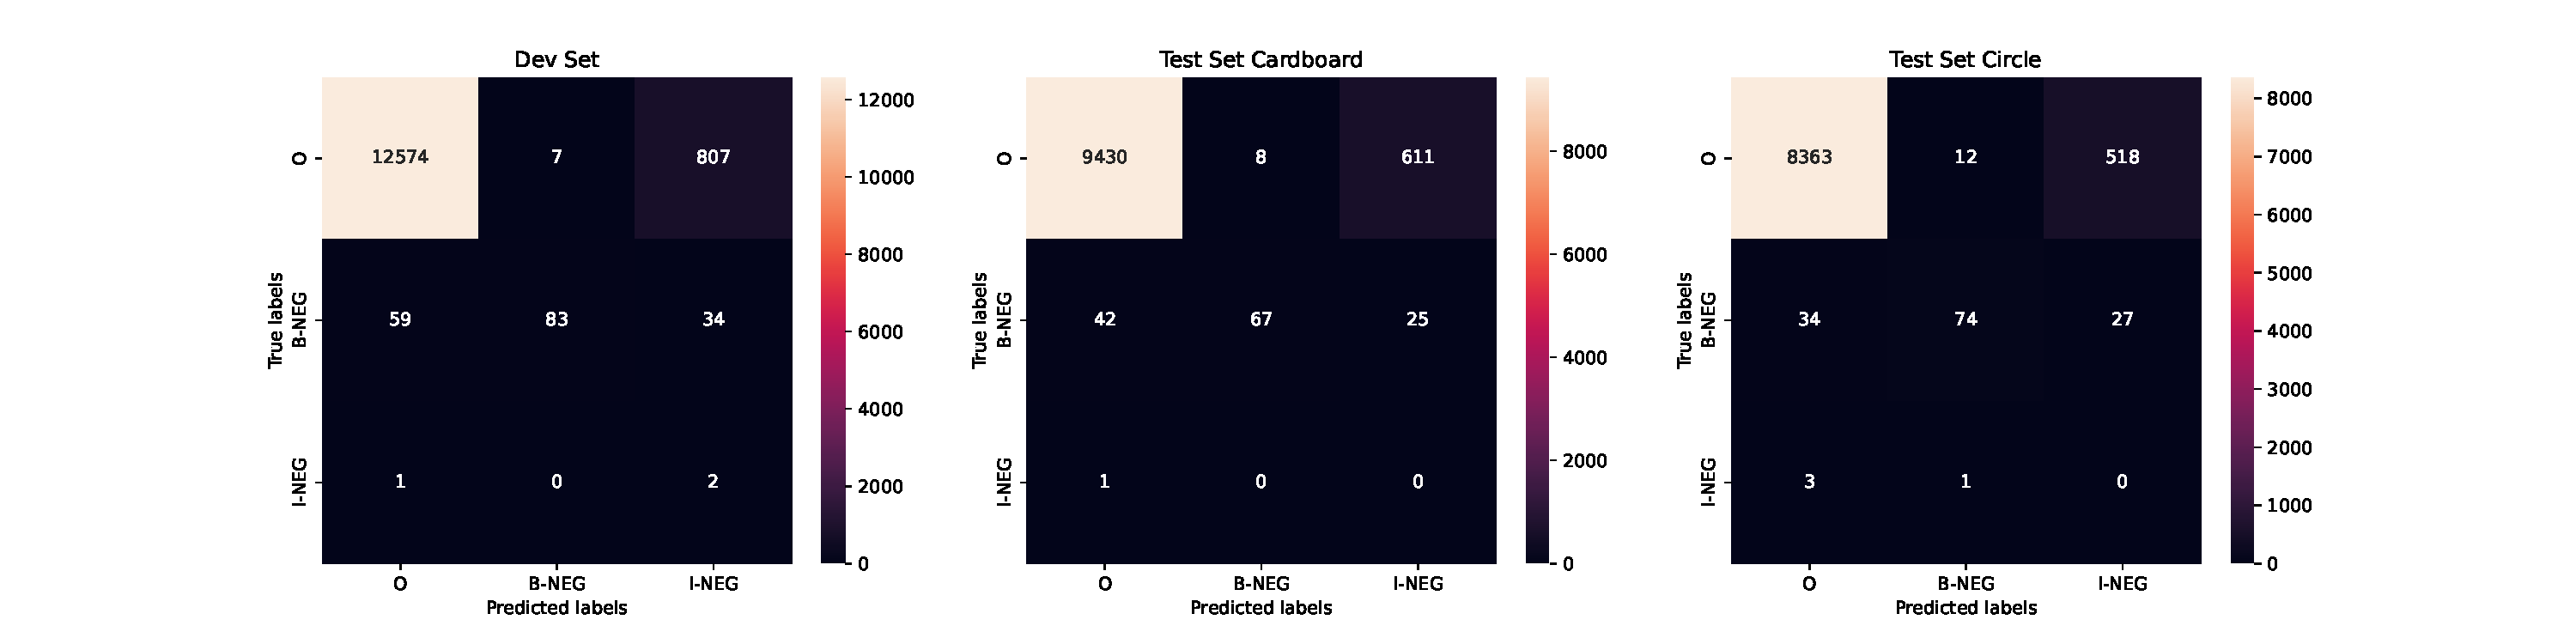
\includegraphics[width=1.3\textwidth]{python_and_notebooks/Plots_and_results//Confusion_Matrix_base_svm.pdf}}
  \caption{Confusion Matrices Baseline SVM}
  \label{fig:base_line_svm}
\end{figure}

In an experiment designed to establish a baseline, the predictive efficacy of the token feature is assessed in isolation. In table \ref{tab:baselines_results}, the results of the baseline are depicted. It can be seen that both weighted F1-score and macro F1-score are around 0.9 and 0.5 respectively for all test sets. Figures \ref{fig:base_line_svm} and \ref{fig:base_line_xgb} shows the confusion matrices of both SVM and XGBoost on the tests and dev sets, providing a further insight into the performance with the feature token alone, it can be seen that despite not having features with contextual information, both classifiers were able to perform reasonably well.
\begin{table}[!ht]
    \centering
    \caption{Classification Report Baseline}
    \label{tab:baselines_results}
\begin{tabular}{lccc|cccr}
\hline
Dataset & \begin{tabular}[c]{@{}l@{}}Precision\\ (SVM)\end{tabular} & \begin{tabular}[c]{@{}l@{}}Recall\\ (SVM)\end{tabular} & \begin{tabular}[c]{@{}l@{}}F1-Score\\ (SVM)\end{tabular} & \begin{tabular}[c]{@{}l@{}}Precision\\ (XGBoost)\end{tabular} & \begin{tabular}[c]{@{}l@{}}Recall\\ (XGBoost)\end{tabular} & \begin{tabular}[c]{@{}l@{}}F1-Score\\ (XGBoost)\end{tabular} & Support  \\
\hline
\textbf{Cardboard} &        &        &        &       &       &       &    \\
O                  &  0.995 &  0.938 &  0.966 & 0.996 & 0.938 & 0.966 & 10049 \\
B-NEG              &  0.893 &  0.500 &  0.641 & 0.897 & 0.522 & 0.660 & 134 \\
I-NEG              &  0.000 &  0.000 &  0.000 & 0.000 & 0.000 & 0.000 & 1 \\
macro avg          &  0.630 &  0.479 &  0.536 & 0.631 & 0.487 & 0.542 & 10184 \\
weighted avg       &  0.994 &  0.933 &  0.962 & 0.994 & 0.933 & 0.962 & 10184 \\
\hline
\textbf{Circle}    &        &        &        &       &       &       &   \\
O                  &  0.996 &  0.940 &  0.967 & 0.996 & 0.940 & 0.967 & 8893 \\
B-NEG              &  0.851 &  0.548 &  0.667 & 0.851 & 0.548 & 0.667 & 135 \\
I-NEG              &  0.000 &  0.000 &  0.000 & 0.000 & 0.000 & 0.000 & 4 \\
macro avg          &  0.615 &  0.496 &  0.545 & 0.615 & 0.496 & 0.545 & 9032 \\
weighted avg       &  0.993 &  0.934 &  0.962 & 0.993 &  0.934 & 0.962 & 9032 \\
\hline
\textbf{Dev set}   &        &        &        &       &       &       &   \\
O                  &  0.995 &  0.939 &  0.966 & 0.996 & 0.939 & 0.967 & 13388 \\
B-NEG              &  0.922 &  0.472 &  0.966 & 0.928 & 0.511 & 0.967 & 176 \\
I-NEG              &  0.002 &  0.667 &  0.005 & 0.002 & 0.667 & 0.005 & 3 \\
macro avg          &  0.640 &  0.692 &  0.532 & 0.642 & 0.706 & 0.544 & 13567 \\
weighted avg       &  0.994 &  0.933 &  0.962 & 0.995 & 0.934 & 0.962 & 13567 \\
\hline
\end{tabular}
\end{table}






Furthermore, the hyperparameters selected for XGBoost were $colsample \ bytree = 0.6$, $learning \ rate = 0.3$, and $max \ depth = 3$ while for SVM, the parameters were $C = 10.0$, $\gamma = 0.5$, and kernel type was set to polynomial based on the grid search results in this particular experiment.

\begin{figure}[!h]
\centering
    \makebox[\textwidth][c]{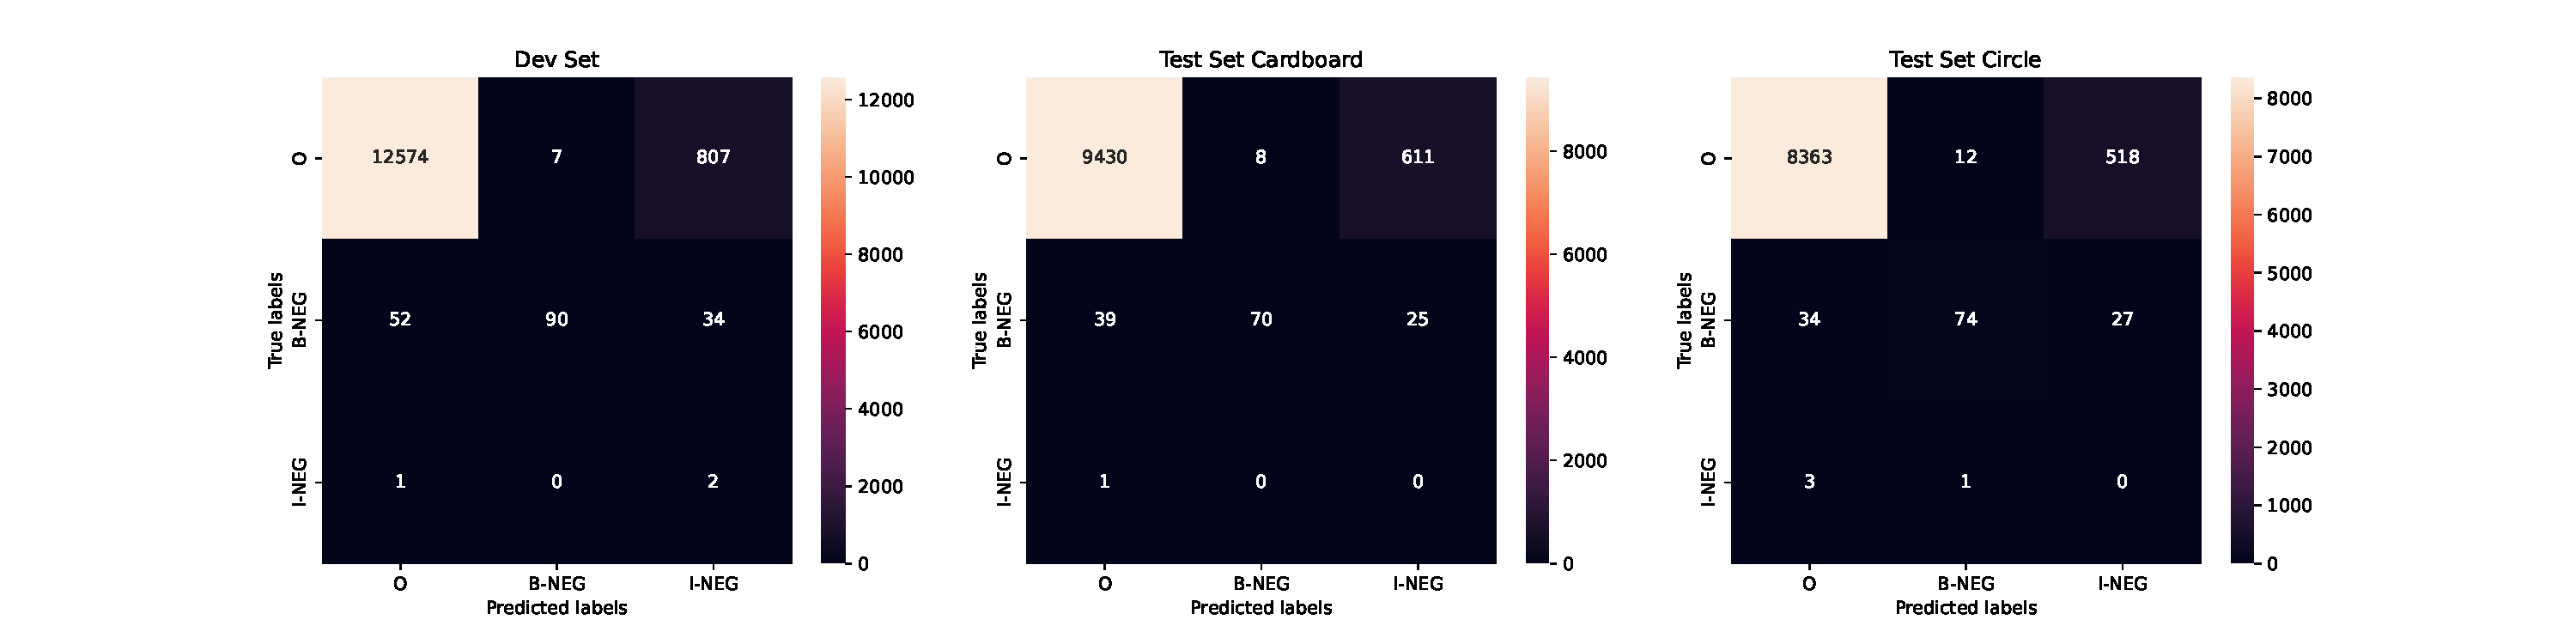
\includegraphics[width=1.3\textwidth]{python_and_notebooks/Plots_and_results//Confusion_Matrix_base_xgb.pdf}}
  \caption{Confusion Matrices Baseline XGBoost}
  \label{fig:base_line_xgb}
\end{figure}
\subsection{Classification Experiments}

During the ablation study, a random feature was removed at each iteration, and the performance of the classifiers was evaluated. The best-performing iterations, denoted as iteration 1 for SVM (SVM 1) and iteration 2 for XGBoost (XGBoost 2), were selected based on their weighted F1-score, which provides a harmonic-weighted average of precision and recall. The weighted F1-score is an appropriate choice as it considers both the balance between precision and recall and the contribution of each class, making it suitable for evaluating classification performance in the presence of imbalanced datasets.

\begin{figure}[!ht]
\centering
    \makebox[\textwidth][c]{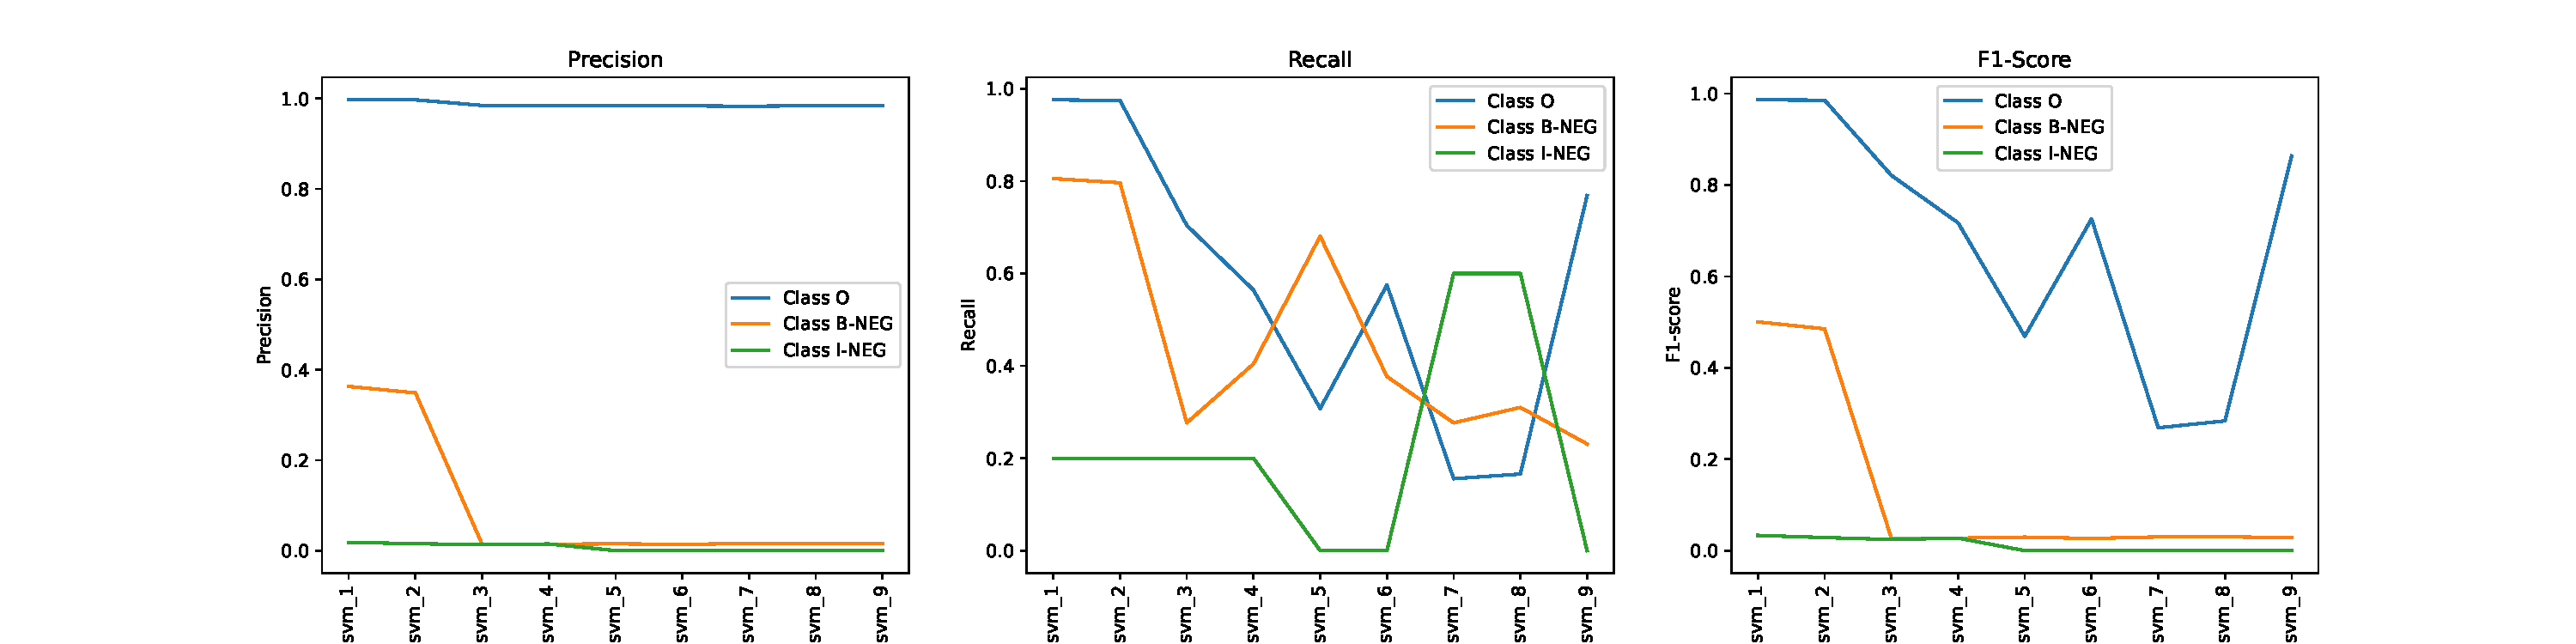
\includegraphics[width=1.3\textwidth]{python_and_notebooks/Plots_and_results//metrics_svm_training.pdf}}
  \caption{Metrics During Ablation Study SVM}
  \label{fig:metrics_svm_training}
\end{figure}

Table \ref{tab:results} presents the classification reports for the best-performing Support Vector Machine (SVM) and XGBoost iterations. Notably, the removal of the feature Token had a remarkable impact on the performance of the classifiers, as evident from the observed drop in F1-scores in Figures \ref{fig:metrics_svm_training} and \ref{fig:metrics_xgb_training}, this drop in performance is completely understandable since the feature "token" is the negation cue itself. By examining the weighted F1-scores and confusion matrices in figures \ref{fig:best_svm} and \ref{fig:best_xgb}, it can be inferred that the SVM classifier slightly outperformed the XGBoost classifier, correctly classifying more data points. However, the SVM classifier failed to classify the minority class "I-NEG" accurately in the development set.

\begin{table}[!ht]
    \centering
    \caption{Classification Report Best Performing Model}
    \label{tab:results}
\begin{tabular}{lccc|cccr}
\hline
Dataset & \begin{tabular}[c]{@{}l@{}}Precision\\ (SVM 1)\end{tabular} &    \begin{tabular}[c]{@{}l@{}}Recall\\ (SVM 1)\end{tabular} &  \begin{tabular}[c]{@{}l@{}}F1-Score\\ (SVM 1)\end{tabular} & \begin{tabular}[c]{@{}l@{}}Precision\\ (XGBoost 2)\end{tabular} &    \begin{tabular}[c]{@{}l@{}}Recall\\ (XGBoost 2)\end{tabular} &  \begin{tabular}[c]{@{}l@{}}F1-Score\\ (XGBoost 2)\end{tabular} & Support  \\
\hline
\textbf{Cardboard} &        &        &        &       &       &       &    \\
O                  & 0.996  &  0.978 & 0.987  & 0.995 & 0.967 & 0.981 & 10049 \\
B-NEG              &  0.342 &  0.731 & 0.466  & 0.244 & 0.686 & 0.360 & 134 \\
I-NEG              &  0.000 &  0.000 &  0.000 & 0.000 & 0.000 & 0.000 & 1 \\
macro avg          &  0.446 &  0.570 &  0.484 & 0.413 & 0.551 & 0.447 & 10184 \\
weighted avg       &  0.987 &  0.975 &  0.980 & 0.985 & 0.963 & 0.973 & 10184 \\
\hline
\textbf{Circle}    &        &        &        &       &       &       &   \\
O                  &  0.996 &  0.974 &  0.985 & 0.995 & 0.959 & 0.977 & 8893 \\
B-NEG              &  0.336 &  0.785 &  0.471 & 0.220 & 0.718 & 0.337 & 135 \\
I-NEG              &  0.000 &  0.000 &  0.000 & 0.000 & 0.000 & 0.000 & 4 \\
macro avg          &  0.444 &  0.586 &  0.485 & 0.405 & 0.559 & 0.438 & 9032 \\
weighted avg       &  0.986 &  0.971 &  0.972 & 0.984 & 0.955 & 0.9672 & 9032 \\
\hline
\textbf{Dev set}   &        &        &        &       &       & &   \\
O                  &  0.995 &  0.980 &  0.988 & 0.995 & 0.969 & 0.982 & 13388 \\
B-NEG              &  0.340 &  0.704 &  0.988 & 0.228 & 0.664 & 0.982 & 176 \\
I-NEG              &  0.000 &  0.000 &  0.000 & 0.043 & 0.333 & 0.076 & 3 \\
macro avg          &  0.445 &  0.561 &  0.482 & 0.422 & 0.655 & 0.466 & 13567 \\
weighted avg       &  0.987 &  0.976 &  0.981 & 0.985 & 0.964 & 0.973 & 13567 \\
\hline
\end{tabular}
\small

{Note:} SVM 1 and XGBoost 2 are for SVM iteration 1 and XGBoost iteration 2 of the ablation study. Table \ref{tab:ablation} presents the features with which these algorithms were trained.
\end{table}



\begin{figure}[!ht]
\centering
    \makebox[\textwidth][c]{\includegraphics[width=1.3\textwidth]{python_and_notebooks/Plots_and_results//metrics_xgb_training.pdf}}
  \caption{Metrics During Ablation Study XGBoost}
  \label{fig:metrics_xgb_training}
\end{figure}

The optimal hyperparameters for the SVM and XGBoost classifiers were determined using grid search. For the SVM classifier, the best parameters were found to be: $ C = 1.0 $, $ \gamma = 1 $, and $ kernel = linear $.  For the XGBoost classifier, the optimal parameters were: $col \ sample \ bytree= 1.0$, $learning \ rate = 0.1$, and $max \ depth = 5$.

Comparing these results to the baseline, the results indicate that, in terms of weighted F1-score, the token feature alone performed slightly worse, which suggests that the inclusion of additional features was a beneficial modification. A closer examination of the confusion matrices reveals an increased number of accurate predictions for the majority classes in the dataset, when adding the extra features. However, he token feature alone demonstrated higher performance at the macro F1-score level.